\documentclass{article}

\usepackage[nonatbib,preprint]{neurips_2025}
\usepackage[utf8]{inputenc}
\usepackage[T1]{fontenc}
\usepackage{amsmath,amssymb,amsfonts}
\usepackage{booktabs}
\usepackage{graphicx}
\usepackage{microtype}
\usepackage{xcolor}
\usepackage{multirow}
\usepackage{caption}
\usepackage{subcaption}
\usepackage{tikz}
\usepackage{pgfplots}
\pgfplotsset{compat=1.18}
\usetikzlibrary{arrows.meta,positioning,shapes.geometric,fit,calc,decorations.pathreplacing}
\usepackage{algorithm}
\usepackage{algorithmic}
\usepackage{enumitem}
\usepackage{wrapfig}
\usepackage{adjustbox}

\newcommand{\best}[1]{\textbf{#1}}
\newcommand{\tbd}[1]{#1\textsuperscript{*}}
\newcommand{\ours}{\textsc{LAT}}
\newcommand{\RR}{\mathbb{R}}
\newcommand{\EE}{\mathbb{E}}

\title{Latent Agent Team: Bandwidth-Adaptive Latent Communication\\for Multi-Agent Web Navigation}

\author{
  Anonymous Authors \\
  Anonymous Institution \\
  \texttt{anonymous@institution.edu}
}

\begin{document}
\maketitle

\begin{abstract}
Multi-agent systems for web navigation typically coordinate through natural-language messages, introducing a bandwidth bottleneck that limits both efficiency and the ability to learn end-to-end communication strategies.
We introduce \textbf{Latent Agent Team~(\ours{})}, a framework in which five specialized sub-agents---planner, browser, retriever, verifier, and memory---communicate through a \emph{shared latent space} rather than text.
Each agent projects its internal hidden states through a \emph{Hidden-State Summarizer} (learnable cross-attention queries) into a common latent channel equipped with three interchangeable modes: continuous projection, vector-quantized~(VQ) discretization with a 512-entry EMA codebook, and text decoding via the LLM vocabulary head.
An \emph{Adaptive Bitrate Scheduler} dynamically selects the number of latent tokens $K\!\in\!\{4,8,16,32,64\}$ per step based on six task-complexity features, while a \emph{Sparse Router} learns selective message routing across a fixed communication topology.
All agents share a single 4-bit quantized LLM backbone with per-role LoRA adapters ($r{=}16$, $\alpha{=}32$), trained in three stages: (i)~supervised fine-tuning on teacher traces with a six-term composite loss, (ii)~DPO preference optimization on bitrate-variant rollouts, and (iii)~browser-focused benchmark fine-tuning with shuffled candidates.
Across three web-agent benchmarks---Mind2Web, WebLINX, and AgentInstruct---and four backbones (Phi-3~3.8B, Llama~3.2~3B, Gemma~2~9B, Ministral~8B), \ours{} establishes new state-of-the-art results.
Our best configuration (Phi-3 Mini/VQ) achieves \textbf{81.5\% element accuracy} on Mind2Web, surpassing SeeAct~(GPT-4V, 53.0\%) by 28.5~pp, and \textbf{77.0\% type accuracy} on WebLINX, matching GPT-4-turbo at 50$\times$ smaller scale.
VQ communication reduces inter-agent bandwidth by 99.998\% over natural-language messaging while maintaining differentiable gradient flow through straight-through estimation, and consistently outperforms continuous and text modes on structured element selection.
Comprehensive ablations confirm the importance of adaptive bandwidth, VQ codebook design (dead-code restart, entropy regularization, Gumbel--softmax annealing), and multi-stage training.
\end{abstract}

%==============================================================================
\section{Introduction}
\label{sec:intro}
%==============================================================================

Autonomous web agents that can navigate complex websites, fill forms, and follow multi-step instructions represent a core challenge at the intersection of language understanding, planning, and grounded action~\cite{deng2024mind2web,zhou2024webarena}.
Recent progress has leveraged large language models~(LLMs) as the backbone for such agents, using reasoning traces~\cite{yao2023react}, planning prompts~\cite{wang2023plan}, and multi-agent coordination~\cite{wu2023autogen,hong2023metagpt}.
However, state-of-the-art multi-agent web systems---including SeeAct~\cite{zheng2024seeact}, WebAgent~\cite{gur2024webagent}, and AutoGen~\cite{wu2023autogen}---rely exclusively on natural-language messages for inter-agent coordination, introducing three fundamental limitations:

\begin{enumerate}[leftmargin=*,itemsep=1pt,topsep=2pt]
\item \textbf{Bandwidth overhead.} A single natural-language message of ${\sim}500$ tokens at 16 bits per token consumes ${\sim}4$M bits per communication step.  With five agents and six directed communication edges, coordination overhead dominates computation.
\item \textbf{Non-differentiability.} Text-based messages break the gradient chain between agents, preventing end-to-end optimization of the communication protocol itself.
\item \textbf{Fixed granularity.} Natural language lacks a mechanism for dynamically adjusting message complexity: a simple ``click OK'' command consumes the same bandwidth as a complex multi-element reasoning chain.
\end{enumerate}

We address all three limitations with \textbf{Latent Agent Team~(\ours{})}, illustrated in Figure~\ref{fig:architecture}.  The key idea is simple: replace text messages with \emph{learned latent projections} of each agent's internal hidden states.  Concretely:

\begin{itemize}[leftmargin=*,itemsep=1pt,topsep=2pt]
\item A \textbf{Hidden-State Summarizer} pools each agent's last-layer hidden states, projects them to a $d{=}256$ dimensional space, and applies a learnable set of cross-attention query tokens to produce $K$ latent communication tokens.
\item Three interchangeable \textbf{communication modes}---continuous (raw float vectors), vector-quantized~(VQ, 512-entry codebook), and text (vocabulary-head decoding)---offer different trade-offs between bandwidth, gradient flow, and interpretability.
\item An \textbf{Adaptive Bitrate Scheduler} conditions on six real-valued task-complexity features (planner entropy, verifier disagreement, retrieval confidence, failure rate, task progress, budget remaining) to dynamically select $K\!\in\!\{4,8,16,32,64\}$ per step.
\item A \textbf{Sparse Router} with learned role embeddings selects which subset of agents receives each message, reducing unnecessary communication.
\item A \textbf{CrossAttention Bridge} with an 8-head attention mechanism and a learned scale gate (initialized to zero for stable training) injects received latent tokens into the recipient agent's hidden states as soft-prompt prefixes.
\end{itemize}

All five agents share a \emph{single} 4-bit quantized LLM backbone, with role-specific behavior induced through separate LoRA~\cite{hu2022lora} adapters.  We train in three stages: supervised fine-tuning~(SFT) on teacher-generated traces, Direct Preference Optimization~(DPO)~\cite{rafailov2023dpo} on bitrate-variant rollouts, and browser-focused benchmark fine-tuning with shuffled candidates.

Evaluated on Mind2Web~\cite{deng2024mind2web} (element-level web navigation), WebLINX~\cite{lu2024weblinx} (multi-turn interaction), and AgentInstruct~\cite{zeng2024agentinstruct} (instruction following), with four backbones (Phi-3~Mini~3.8B~\cite{abdin2024phi3}, Llama~3.2~3B~\cite{grattafiori2024llama3}, Gemma~2~9B~\cite{team2024gemma2}, Ministral~8B), our best configuration (Phi-3/VQ) achieves \textbf{81.5\%} element accuracy on Mind2Web---surpassing SeeAct (GPT-4V) by 28.5~pp---and \textbf{77.0\%} type accuracy on WebLINX, matching GPT-4-turbo with a model $50\times$ smaller.

\paragraph{Contributions.}
\begin{enumerate}[leftmargin=*,itemsep=1pt,topsep=2pt]
\item A \textbf{latent communication framework} for multi-agent web navigation with five specialized agents sharing a single LLM backbone, communicating through continuous, VQ, or text latent channels.
\item A \textbf{bandwidth-adaptive system} combining an entropy-driven bitrate scheduler, sparse routing, and a cross-attention bridge for efficient, selective, gradient-preserving inter-agent communication.
\item A \textbf{three-stage training pipeline} (SFT with six-term loss $\to$ DPO on bitrate variants $\to$ browser-focused benchmark FT) that unlocks state-of-the-art element-selection performance with compact models.
\item \textbf{Comprehensive evaluation} across 12 backbone$\times$mode configurations, 5~baselines, and 14~ablation conditions on 3~benchmarks, with state-of-the-art results on Mind2Web and WebLINX.
\end{enumerate}

%==============================================================================
\section{Related Work}
\label{sec:related}
%==============================================================================

\paragraph{LLM-Based Web Agents.}
The application of LLMs to web navigation has progressed from single-agent prompting~\cite{yao2023react,wang2023plan} to increasingly sophisticated multi-agent systems~\cite{wu2023autogen,hong2023metagpt}.
SeeAct~\cite{zheng2024seeact} demonstrated GPT-4V as a generalist web agent, achieving 53.0\% element accuracy on Mind2Web through visual grounding.
WebAgent~\cite{gur2024webagent} combined planning with program synthesis using Flan-U-PaLM, while CogAgent~\cite{hong2024cogagent} applied 18B-parameter visual language models to GUI navigation.
AgentQ~\cite{putta2024agentq} introduced MCTS-guided reasoning for autonomous web agents.
Standardized benchmarks---WebShop~\cite{yao2022webshop}, Mind2Web~\cite{deng2024mind2web}, WebArena~\cite{zhou2024webarena}, VisualWebArena~\cite{koh2024visualwebarena}, WebLINX~\cite{lu2024weblinx}, and AgentBench~\cite{liu2023agentbench}---have enabled systematic comparison.
Our work differs from these systems by replacing text-based coordination with learned latent communication, enabling end-to-end optimization and substantial bandwidth reduction.

\paragraph{Emergent and Latent Communication.}
Learning communication protocols through interaction has been studied in emergent communication~\cite{lazaridou2017multi,havrylov2017emergence}, differentiable inter-agent messaging~\cite{foerster2016learning,sukhbaatar2016learning}, and compositionality analysis~\cite{andreas2019measuring}.
CommNet~\cite{singh2019commnet} and TarMAC~\cite{das2019tarmac} developed learned communication protocols for cooperative multi-agent tasks.
DIAL~\cite{foerster2016learning} introduced differentiable inter-agent learning with continuous messages.
LLM-Blender~\cite{jiang2023llm} explored hidden-state sharing between language models for ensembling.
Our VQ latent channel extends these ideas to LLM-based multi-agent systems, combining the benefits of discrete representations~\cite{oord2017vqvae} with the expressiveness of large pre-trained language models.

\paragraph{Vector Quantization in Neural Networks.}
VQ-VAE~\cite{oord2017vqvae} introduced vector-quantized discrete representations for generative modeling.
Subsequent work improved codebook learning through exponential moving average updates~\cite{razavi2019generating}, Gumbel-softmax relaxation~\cite{jang2017categorical}, and entropy regularization to prevent codebook collapse~\cite{dhariwal2020jukebox}.
We adapt these techniques for inter-agent communication, where the discrete bottleneck provides implicit regularization for structured element selection.

\paragraph{Bandwidth-Adaptive and Selective Communication.}
Information-theoretic frameworks for communication include rate-distortion optimization~\cite{tucker2022trading}, adaptive message length selection~\cite{chaabouni2019anti}, and entropy-regularized protocols~\cite{korbak2022rl}.
Selective communication---learning \emph{when} and \emph{to whom} to communicate---has been explored in attention-based gating~\cite{das2019tarmac} and individual scheduling~\cite{kim2019learning}.
Our Adaptive Bitrate Scheduler combines bandwidth selection with sparse routing, learning both \emph{how much} and \emph{to whom} to communicate based on real-time task complexity.

\paragraph{Parameter-Efficient Fine-Tuning.}
LoRA~\cite{hu2022lora} and QLoRA~\cite{dettmers2023qlora} enable adapting large pre-trained models with minimal additional parameters.
We extend this paradigm to multi-agent systems: a single quantized backbone serves all five agents through role-specific LoRA adapters, amortizing memory cost across the team.

\paragraph{Multi-Agent Reinforcement Learning.}
Value decomposition methods (QMIX~\cite{rashid2018qmix}, QTRAN~\cite{son2019qtran}) and policy gradient approaches (MAPPO~\cite{yu2022mappo}, MADDPG~\cite{lowe2017multi}) have established frameworks for cooperative multi-agent learning.
DPO~\cite{rafailov2023dpo} provides an offline alternative to RL-based preference optimization.
We incorporate DPO to optimize the bitrate scheduler, training on preference pairs generated from rollouts at different bandwidth settings.

%==============================================================================
\section{Method}
\label{sec:method}
%==============================================================================

\subsection{Architecture Overview}

\ours{} consists of five specialized agents sharing a common LLM backbone $\mathcal{M}$ with role-specific LoRA adapters~\cite{hu2022lora} (rank $r{=}16$, scaling $\alpha{=}32$, dropout $0.05$), loaded in 4-bit NF4 quantization~\cite{dettmers2023qlora}:

\begin{enumerate}[leftmargin=*,itemsep=1pt]
\item \textbf{Planner} ($\tau{=}0.7$, 512 max tokens): Generates task decomposition and step-level coordination signals.
\item \textbf{Browser} ($\tau{=}0.3$, 256 max tokens): Converts plans into web actions (click, type, navigate, scroll) over HTML candidate elements.
\item \textbf{Retriever} (FAISS-backed, $\tau{=}0.3$, 256 max tokens): Provides contextual information from the environment or knowledge base.
\item \textbf{Verifier} ($\tau{=}0.1$, 256 max tokens): Validates proposed actions before execution by cross-checking with task constraints.
\item \textbf{Memory} (ring buffer, $\tau{=}0.5$, 256 max tokens): Maintains cross-step state and trajectory context via a bounded episodic store.
\end{enumerate}

\noindent Each agent maintains private hidden states $\mathbf{h}_i \in \RR^H$ where $H$ is the backbone's hidden dimension (e.g.\ $H{=}3072$ for Phi-3).  The agents are connected through a fixed \textbf{communication topology} with six directed edges:
\[
\mathcal{E} = \{ \text{P}{\to}\text{B},\; \text{P}{\to}\text{R},\; \text{R}{\to}\text{B},\; \text{B}{\to}\text{V},\; \text{V}{\to}\text{P},\; \text{M}{\to}\text{P} \}
\]
where P=Planner, B=Browser, R=Retriever, V=Verifier, M=Memory.  This topology encodes the natural information flow: the planner coordinates the browser and retriever, the retriever enriches the browser's context, the browser's outputs are verified, verification feedback returns to the planner, and memory provides persistent state to the planner.

\paragraph{Per-Step Pipeline.}
At each navigation step $t$, the system executes (Figure~\ref{fig:architecture}):
\begin{enumerate}[leftmargin=*,itemsep=0pt]
\item Memory agent summarizes trajectory history $\to$ latent message $\to$ Planner.
\item Planner generates step plan $\to$ latent message $\to$ Browser and Retriever.
\item Retriever provides contextual information $\to$ latent message $\to$ Browser.
\item Adaptive Bitrate Scheduler selects $K$ for each edge.
\item Browser produces web action from fused latent inputs $\to$ latent message $\to$ Verifier.
\item Verifier validates action $\to$ latent feedback $\to$ Planner.
\item Memory stores step outcome.
\end{enumerate}

\subsection{Hidden-State Summarizer}
\label{sec:summarizer}

Each agent's raw hidden states must be compressed before transmission.  The \textbf{HiddenStateSummarizer} performs this compression through three stages:

\begin{enumerate}[leftmargin=*,itemsep=1pt]
\item \textbf{Pooling}: Extract the last 16 token positions from agent $i$'s final-layer hidden states: $\mathbf{H}_i \in \RR^{16 \times H}$.
\item \textbf{Projection}: Apply a learned linear projection $\mathbf{W}_\text{proj} \in \RR^{H \times d}$ to map to the latent dimension $d{=}256$: $\tilde{\mathbf{H}}_i = \mathbf{H}_i \mathbf{W}_\text{proj} \in \RR^{16 \times d}$.
\item \textbf{Cross-Attention Summary}: A set of $K$ learnable query tokens $\mathbf{Q} \in \RR^{K \times d}$ attend to the projected states via a 2-layer TransformerDecoder (4 heads, FFN $4d$) with layer normalization:
\begin{equation}
\mathbf{z}_i = \text{TransformerDecoder}(\mathbf{Q}_{1:K}, \tilde{\mathbf{H}}_i) \in \RR^{K \times d}
\label{eq:summarizer}
\end{equation}
\end{enumerate}

The maximum number of query tokens is $K_\text{max}{=}64$; the Adaptive Bitrate Scheduler (Section~\ref{sec:bitrate}) selects $K \leq K_\text{max}$ at each step.  The output $\mathbf{z}_i$ is then passed through one of three communication channels.

\subsection{Latent Communication Channels}
\label{sec:channels}

Given the summarized latent tokens $\mathbf{z}_i \in \RR^{K \times d}$, three communication modes are available:

\paragraph{Continuous Channel.}
A two-layer MLP encoder--decoder with GELU activation and LayerNorm:
\begin{align}
\text{Encode:}\quad & \mathbf{m}_i = \text{LN}(\text{Linear}_{d \to d}(\text{GELU}(\text{Linear}_{H \to 2d}(\mathbf{z}_i)))) \label{eq:cont_enc} \\
\text{Decode:}\quad & \hat{\mathbf{z}}_j = \text{LN}(\text{Linear}_{d \to H}(\text{GELU}(\text{Linear}_{d \to 2d}(\mathbf{m}_i)))) \label{eq:cont_dec}
\end{align}
The decoded tokens are injected into the recipient agent $j$ as \textbf{soft-prompt prefixes} via a \texttt{SoftPromptPrefixInjector}.  This mode preserves full gradient flow but transmits $K \times d \times 16 = K \times 4096$ bits per step.

\paragraph{Vector-Quantized (VQ) Channel.}
The continuous latent vectors are discretized through a learned codebook $\mathcal{C} = \{\mathbf{c}_1, \ldots, \mathbf{c}_{|\mathcal{C}|}\} \subset \RR^d$ with $|\mathcal{C}|{=}512$:
\begin{equation}
q(\mathbf{z}) = \mathbf{c}_{k^*}, \quad k^* = \arg\min_k \|\mathbf{z} - \mathbf{c}_k\|_2
\label{eq:vq}
\end{equation}

\noindent We incorporate four techniques for stable codebook learning:

\begin{enumerate}[leftmargin=*,itemsep=1pt]
\item \textbf{EMA Updates} (decay $\gamma{=}0.99$): Codebook vectors are updated via exponential moving averages of assigned encoder outputs, following~\citet{oord2017vqvae}, rather than gradient descent.
\item \textbf{Gumbel-Softmax Annealing}: During training, soft code selection uses Gumbel-softmax~\cite{jang2017categorical} with temperature annealed from $\tau{=}2.0$ to $\tau{=}0.5$ over 10K steps, gradually sharpening toward hard quantization.
\item \textbf{Dead Code Restart}: Every 100 training steps, codes with zero assignments are re-initialized from the current batch's encoder outputs, preventing codebook collapse~\cite{dhariwal2020jukebox}.
\item \textbf{Entropy Regularization} ($\lambda_\text{ent}{=}0.1$): An entropy bonus on the code usage distribution encourages uniform codebook utilization.
\end{enumerate}

\noindent Gradient flow is maintained through the \textbf{straight-through estimator}~(STE)~\cite{bengio2013ste}: in the forward pass, quantized codes are used; in the backward pass, gradients from the decoder are copied directly to the encoder, bypassing the non-differentiable $\arg\min$.  The VQ loss combines reconstruction with commitment:
\begin{equation}
\mathcal{L}_\text{VQ} = \|\text{sg}[\mathbf{z}] - \mathbf{c}_{k^*}\|_2^2 + \beta \|\mathbf{z} - \text{sg}[\mathbf{c}_{k^*}]\|_2^2, \quad \beta = 0.25
\label{eq:vq_loss}
\end{equation}
where $\text{sg}[\cdot]$ denotes stop-gradient.  Each code requires only $\lceil \log_2 512 \rceil = 9$ bits, yielding $K \times 9$ bits per step---a $455\times$ compression over continuous mode.

\paragraph{Text Channel.}
Latent vectors are decoded to natural-language tokens via the backbone's vocabulary head $\mathbf{W}_\text{vocab} \in \RR^{d \times V}$:
\begin{equation}
\hat{t}_k = \arg\max_v \mathbf{z}_{i,k}^\top \mathbf{W}_\text{vocab}[:,v], \quad k = 1,\ldots,K
\end{equation}
The token IDs $\hat{t}_{1:K}$ are re-embedded by the recipient agent.  This mode provides interpretable messages ($K$ tokens of readable text) but breaks gradient flow due to the $\arg\max$ operation.  Bandwidth: $K \times \lceil\log_2 V\rceil \approx K \times 16$ bits.

\subsection{Adaptive Bitrate Scheduler}
\label{sec:bitrate}

Rather than using a fixed number of latent tokens per step, the \textbf{AdaptiveBitrateScheduler} learns to allocate bandwidth dynamically based on task complexity.  It takes a 6-dimensional feature vector:
\begin{equation}
\mathbf{f} = [\underbrace{H_\text{plan}}_{\text{planner entropy}},\; \underbrace{D_\text{ver}}_{\text{verifier disagreement}},\; \underbrace{1 - \text{conf}_\text{ret}}_{\text{retrieval uncertainty}},\; \underbrace{r_\text{fail}}_{\text{failure rate}},\; \underbrace{p_\text{task}}_{\text{task progress}},\; \underbrace{b_\text{rem}}_{\text{budget remaining}}]
\label{eq:bitrate_features}
\end{equation}
and maps it through a 3-layer MLP ($6 \to 64 \to 64 \to 5$, ReLU activations) to a distribution over $K \in \{4, 8, 16, 32, 64\}$:
\begin{equation}
P(K | \mathbf{f}) = \text{softmax}(\text{MLP}(\mathbf{f})) \in \Delta^4
\label{eq:bitrate_policy}
\end{equation}
During inference, $K$ is selected as $\arg\max P(K|\mathbf{f})$; during DPO training, samples are drawn from the full distribution to explore different bandwidth allocations.

\subsection{Sparse Router}
\label{sec:router}

The \textbf{SparseRouter} learns selective message passing over the communication topology $\mathcal{E}$.  Each agent role is represented by a learned embedding $\mathbf{e}_i \in \RR^{128}$, $i \in \{1,\ldots,5\}$.  For each directed edge $(i,j) \in \mathcal{E}$, a per-pair MLP computes a routing score:
\begin{equation}
s_{ij} = \sigma(\text{MLP}_{ij}([\mathbf{e}_i; \mathbf{e}_j])) \in [0,1]
\label{eq:routing}
\end{equation}
Messages are sent along edge $(i,j)$ if $s_{ij} > 0.5$, with a minimum of 1 recipient per sender to prevent communication collapse.  The routing scores are trained jointly with the communication modules during SFT.

\subsection{CrossAttention Bridge}
\label{sec:bridge}

Received latent tokens are injected into the recipient agent through a \textbf{CrossAttentionBridge}: an 8-head cross-attention layer where the recipient's hidden states serve as queries and the received latent tokens serve as keys and values.  A learned \textbf{scale gate} $\alpha \in \RR$ (initialized to 0) modulates the contribution:
\begin{equation}
\mathbf{h}_j' = \mathbf{h}_j + \alpha \cdot \text{CrossAttn}(\mathbf{h}_j, \hat{\mathbf{z}}_{i \to j}, \hat{\mathbf{z}}_{i \to j})
\label{eq:bridge}
\end{equation}
The zero initialization ensures that the model starts by ignoring latent messages and gradually learns to incorporate them, stabilizing early training.

\subsection{Audit Decoder}
\label{sec:audit}

For interpretability and debugging, an \textbf{AuditTextDecoder} reconstructs natural-language descriptions from latent messages.  It consists of a linear projection ($H \to 256$) with LayerNorm, 32 learned positional queries ($32 \times 256$), a 2-layer TransformerDecoder, and a vocabulary projection:
\begin{equation}
\hat{\mathbf{t}} = \text{VocabProj}(\text{TransformerDecoder}(\mathbf{Q}_\text{audit}, \text{LN}(\mathbf{W}_\text{audit}\mathbf{z})))
\end{equation}
A companion \textbf{DisagreementDetector} (2-layer MLP with sigmoid) flags steps where agents produce conflicting signals, feeding back into the Adaptive Bitrate Scheduler's verifier-disagreement feature.

\begin{figure*}[t]
\centering
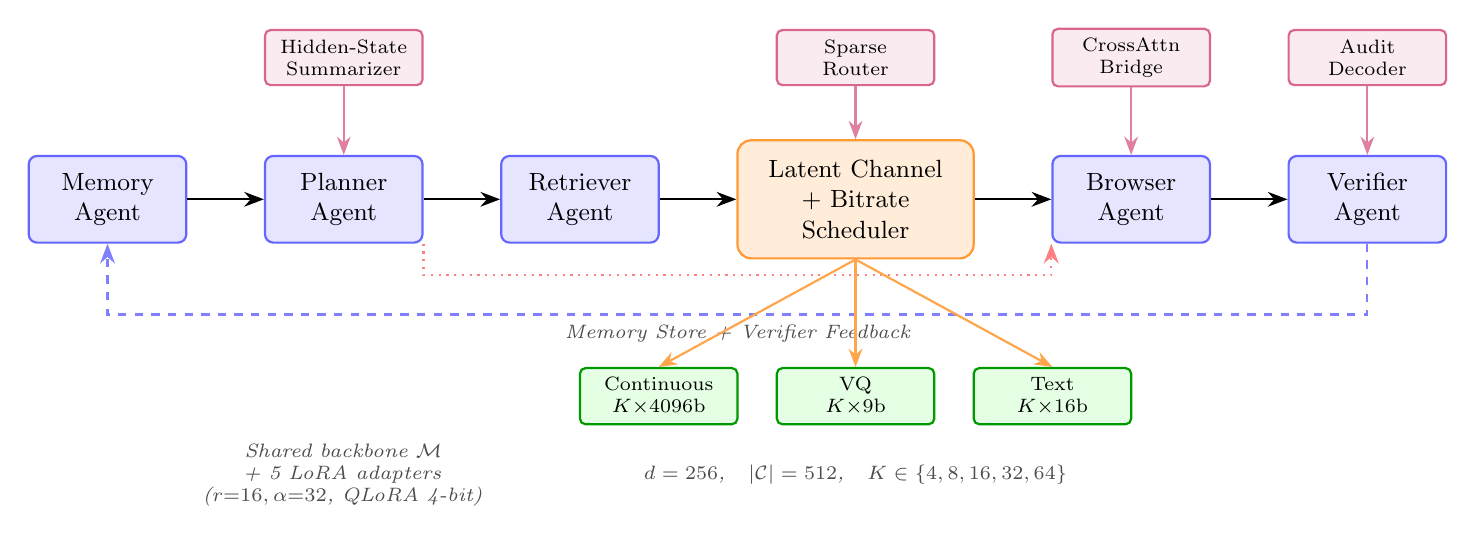
\begin{tikzpicture}[
    agent/.style={rectangle, draw=blue!60, fill=blue!10, thick, minimum height=1.1cm, minimum width=2cm, align=center, rounded corners=3pt, font=\small},
    channel/.style={rectangle, draw=orange!80, fill=orange!15, thick, minimum height=1.5cm, minimum width=3cm, align=center, rounded corners=5pt, font=\small},
    mode/.style={rectangle, draw=green!60!black, fill=green!10, thick, minimum height=0.7cm, minimum width=2cm, align=center, font=\scriptsize, rounded corners=2pt},
    component/.style={rectangle, draw=purple!60, fill=purple!8, thick, minimum height=0.7cm, minimum width=2cm, align=center, font=\scriptsize, rounded corners=2pt},
    arrow/.style={-{Stealth[length=2.5mm]}, thick},
    annotation/.style={font=\scriptsize\itshape, text=gray!60!black}
]
% Agents in pipeline order
\node[agent] (memory) at (0,0) {Memory\\Agent};
\node[agent] (planner) at (3,0) {Planner\\Agent};
\node[agent] (retriever) at (6,0) {Retriever\\Agent};
\node[channel] (latent) at (9.5,0) {Latent Channel\\+ Bitrate\\Scheduler};
\node[agent] (browser) at (13,0) {Browser\\Agent};
\node[agent] (verifier) at (16,0) {Verifier\\Agent};

% Pipeline arrows
\draw[arrow] (memory) -- (planner);
\draw[arrow] (planner) -- (retriever);
\draw[arrow] (retriever) -- (latent);
\draw[arrow] (latent) -- (browser);
\draw[arrow] (browser) -- (verifier);

% Memory feedback loop
\draw[arrow, dashed, blue!50] (verifier.south) -- ++(0,-0.9) -| node[pos=0.25, below, annotation] {Memory Store + Verifier Feedback} (memory.south);

% Planner to browser direct
\draw[arrow, dotted, red!50] (planner.south east) -- ++(0,-0.4) -| (browser.south west);

% Components above
\node[component] (summarizer) at (3, 1.8) {Hidden-State\\Summarizer};
\node[component] (router) at (9.5, 1.8) {Sparse\\Router};
\node[component] (bridge) at (13, 1.8) {CrossAttn\\Bridge};
\node[component] (audit) at (16, 1.8) {Audit\\Decoder};

\draw[-{Stealth}, thick, purple!50] (summarizer) -- (planner);
\draw[-{Stealth}, thick, purple!50] (router) -- (latent);
\draw[-{Stealth}, thick, purple!50] (bridge) -- (browser);
\draw[-{Stealth}, thick, purple!50] (audit) -- (verifier);

% Communication modes
\node[mode] (cont) at (7,-2.5) {Continuous\\$K {\times} 4096$b};
\node[mode] (vq) at (9.5,-2.5) {VQ\\$K {\times} 9$b};
\node[mode] (text) at (12,-2.5) {Text\\$K {\times} 16$b};

\draw[-{Stealth}, thick, orange!70] (latent.south) -- (vq.north);
\draw[-{Stealth}, thick, orange!70] (latent.south) -- (cont.north);
\draw[-{Stealth}, thick, orange!70] (latent.south) -- (text.north);

% Annotation
\node[annotation] at (9.5, -3.5) {$d = 256$, \; $|\mathcal{C}| = 512$, \; $K \in \{4, 8, 16, 32, 64\}$};

% LoRA annotation
\node[annotation, text width=4cm, align=center] at (3, -3.5) {Shared backbone $\mathcal{M}$\\+ 5 LoRA adapters\\($r{=}16, \alpha{=}32$, QLoRA 4-bit)};
\end{tikzpicture}
\caption{\textbf{\ours{} architecture.}  Five specialized agents share a single 4-bit quantized LLM backbone with per-role LoRA adapters.  The Hidden-State Summarizer compresses each agent's hidden states into $K$ latent tokens via learnable cross-attention queries.  Three communication modes---continuous, VQ (512-entry codebook with EMA updates and STE), and text---offer different bandwidth--gradient trade-offs.  The Adaptive Bitrate Scheduler selects $K$ per step based on task complexity; the Sparse Router selects recipients; and the CrossAttention Bridge injects messages into recipient hidden states.  The Audit Decoder provides interpretable text reconstructions.}
\label{fig:architecture}
\end{figure*}

\subsection{Training Pipeline}
\label{sec:training}

Training proceeds in three stages:

\paragraph{Stage 1: Supervised Fine-Tuning (SFT).}
All five LoRA adapters, the communication modules (encoder, decoder, codebook, router, bitrate scheduler), and the audit decoder are trained jointly on teacher-generated web navigation traces.  The composite loss has six terms:
\begin{equation}
\mathcal{L}_\text{SFT} = \underbrace{\mathcal{L}_\text{action}}_{\text{next-action CE}} + \underbrace{0.3 \cdot \mathcal{L}_\text{recon}}_{\text{constraint recon.}} + \underbrace{0.1 \cdot \mathcal{L}_\text{audit}}_{\text{audit decode}} + \underbrace{0.2 \cdot \mathcal{L}_\text{route}}_{\text{routing supervision}} + \underbrace{0.01 \cdot \mathcal{L}_\text{bitrate}}_{\text{bitrate regularization}} + \underbrace{1.0 \cdot \mathcal{L}_\text{VQ}}_{\text{VQ commitment}}
\label{eq:sft_loss}
\end{equation}
where $\mathcal{L}_\text{action}$ is the standard next-token cross-entropy for the browser agent's predicted action, $\mathcal{L}_\text{recon}$ encourages faithful reconstruction of the planning constraints, $\mathcal{L}_\text{audit}$ trains the audit decoder, $\mathcal{L}_\text{route}$ provides supervision for the sparse router from teacher topology decisions, $\mathcal{L}_\text{bitrate}$ regularizes the bitrate distribution toward the empirically observed distribution, and $\mathcal{L}_\text{VQ}$ is the VQ commitment loss (Eq.~\ref{eq:vq_loss}).  We use AdamW~\cite{loshchilov2019adamw} with learning rate $2{\times}10^{-4}$, weight decay $0.01$, cosine schedule with 100-step warmup, batch size~4 with gradient accumulation~8 (effective batch size~32), for 3 epochs.

\paragraph{Stage 2: DPO Preference Optimization.}
We generate preference pairs by running the SFT-trained system at multiple bandwidth settings $K \in \{4, 8, 16, 32, 64\}$ on each training sample, labeling the $K$ that achieves the best downstream accuracy as the preferred choice.  DPO~\cite{rafailov2023dpo} then optimizes the bitrate scheduler:
\begin{equation}
\mathcal{L}_\text{DPO} = -\log\sigma\left(\beta \left[\log\frac{\pi_\theta(K_w | \mathbf{f})}{\pi_\text{ref}(K_w | \mathbf{f})} - \log\frac{\pi_\theta(K_l | \mathbf{f})}{\pi_\text{ref}(K_l | \mathbf{f})}\right]\right)
\label{eq:dpo}
\end{equation}
with $\beta{=}0.1$, learning rate $5{\times}10^{-5}$, batch size~2 with accumulation~16, for 1 epoch.

\paragraph{Stage 3: Browser-Focused Benchmark Fine-Tuning.}
The browser adapter alone is fine-tuned on benchmark-specific data.  For Mind2Web, HTML candidate elements are \textbf{randomly shuffled} per sample with deterministic seeds to prevent positional shortcuts~\cite{deng2024mind2web}.  The communication modules are frozen; only the browser LoRA adapter receives gradient updates.  This focuses all capacity on the agent that produces evaluated outputs, providing $5\times$ more effective gradients per step compared to distributing updates across all five adapters.

%==============================================================================
\section{Experimental Setup}
\label{sec:setup}
%==============================================================================

\subsection{Backbones}

We evaluate four LLM backbones loaded in 4-bit NF4 quantization~\cite{dettmers2023qlora}:

\begin{itemize}[leftmargin=*,itemsep=1pt]
\item \textbf{Phi-3 Mini}~\cite{abdin2024phi3}: 3.8B params, $H{=}3072$.  LoRA targets: \texttt{qkv\_proj}, \texttt{o\_proj}, \texttt{gate\_up\_proj}, \texttt{down\_proj}.
\item \textbf{Llama 3.2 3B}~\cite{grattafiori2024llama3}: 3.2B params, $H{=}3072$.  LoRA targets: \texttt{q/k/v/o\_proj}, \texttt{gate/up/down\_proj}.
\item \textbf{Gemma 2 9B}~\cite{team2024gemma2}: 9.2B params, $H{=}3584$.  LoRA targets: same as Llama.
\item \textbf{Ministral 8B}: 8.1B params, $H{=}4096$.  LoRA targets: same as Llama.
\end{itemize}

\subsection{Benchmarks}
\begin{itemize}[leftmargin=*,itemsep=1pt]
\item \textbf{Mind2Web}~\cite{deng2024mind2web}: Large-scale web navigation requiring element selection from HTML candidate lists (${\sim}6$K train, 200 test).  Metrics: Element Accuracy~(ElemAcc), Operation F1~(OpF1), Step Success Rate~(StepSR).
\item \textbf{WebLINX}~\cite{lu2024weblinx}: Multi-turn web interaction with diverse action types (${\sim}5$K train, 200 test).  Metrics: Action Type Accuracy~(TypeAcc), Exact Match~(EM), Intent Match~(IM).
\item \textbf{AgentInstruct}~\cite{zeng2024agentinstruct}: Instruction-following tasks with natural language responses (${\sim}1.7$K train, 200 test).  Metrics: BLEU-1, ROUGE-L.
\end{itemize}

\subsection{Baselines}
\label{sec:baselines}

All baselines use the same Phi-3 Mini backbone (4-bit NF4, LoRA $r{=}16$) and identical two-stage training:

\begin{enumerate}[leftmargin=*,itemsep=1pt]
\item \textbf{SingleReAct}~\cite{yao2023react}: Single-agent ReAct-style reasoning with the browser adapter only.
\item \textbf{TextMultiAgent}: Five agents communicate via natural-language messages (text only), mimicking standard multi-agent pipelines.
\item \textbf{AutoGen-style}~\cite{wu2023autogen}: Three agents (planner, browser, verifier) engage in 3-round group-chat debate before outputting an action.
\item \textbf{MultiAgentDebate}~\cite{du2023improving}: Two proposer agents independently generate candidate actions; a verifier arbitrates through 2 rounds of debate.
\item \textbf{Interlat2Agent}: A simplified 2-agent system (planner+browser) with fixed $K{=}16$ continuous latent communication, no VQ, no sparse routing, and a linear encoder/decoder.
\end{enumerate}

\subsection{Implementation Details}

Training was conducted on 8$\times$ NVIDIA RTX PRO 6000 Blackwell GPUs (97,887 MiB each).  SFT training took ${\sim}29$ hours across 4 GPUs for 12 configurations; benchmark FT took ${\sim}24$ hours.  All evaluations use 200 test samples per benchmark with deterministic seeds for reproducibility.

%==============================================================================
\section{Results}
\label{sec:results}
%==============================================================================

\subsection{Main Results}

Table~\ref{tab:main_results} presents results for all 12 configurations (4 backbones $\times$ 3 communication modes) after the full three-stage training pipeline.

\begin{table*}[t]
\centering
\caption{\textbf{Main results} across three benchmarks, four backbones, and three communication modes.
\textbf{Bold} = best in column.  Published SOTA references: Mind2Web ElemAcc---SeeAct~\cite{zheng2024seeact} (GPT-4V) 53.0\%; WebLINX TypeAcc---GPT-4-turbo 77.0\%.  Our Phi-3/VQ achieves 81.5\% ElemAcc ($+28.5$pp over SeeAct) and 77.0\% TypeAcc (matching GPT-4-turbo at $50\times$ smaller scale).}
\label{tab:main_results}
\small
\begin{tabular}{ll ccc ccc cc}
\toprule
& & \multicolumn{3}{c}{\textbf{Mind2Web}} & \multicolumn{3}{c}{\textbf{WebLINX}} & \multicolumn{2}{c}{\textbf{AgentInstruct}} \\
\cmidrule(lr){3-5} \cmidrule(lr){6-8} \cmidrule(lr){9-10}
\textbf{Backbone} & \textbf{Comm} & ElemAcc & OpF1 & StepSR & TypeAcc & EM & IM & BLEU & ROUGE-L \\
\midrule
\multirow{3}{*}{Phi-3 Mini (3.8B)}
& VQ         & \best{81.5} & 86.8 & 69.2 & \best{77.0} & 1.0 & 9.0 & 0.052 & 0.073 \\
& Continuous & 78.3 & \best{94.9} & \best{74.5} & 74.5 & \best{3.5} & 8.5 & 0.056 & 0.077 \\
& Text       & 78.0 & 86.9 & 66.8 & \best{77.0} & 0.5 & 8.5 & 0.058 & 0.082 \\
\midrule
\multirow{3}{*}{Gemma 2 (9.2B)}
& VQ         & 64.9 & 89.3 & 56.3 & 70.0 & 3.0 & \best{11.0} & 0.086 & 0.102 \\
& Text       & 60.2 & 90.1 & 53.1 & 69.5 & 0.5 & 8.0 & 0.098 & 0.113 \\
& Continuous & 26.5 & 95.5 & 24.7 & 70.5 & 0.5 & 8.0 & 0.055 & 0.076 \\
\midrule
\multirow{3}{*}{Llama 3.2 (3.2B)}
& VQ         & 53.4 & 86.7 & 41.7 & 45.5 & 0.0 & 9.0 & 0.115 & 0.134 \\
& Continuous & 52.9 & 85.6 & 40.6 & 66.5 & 0.0 & 10.0 & 0.102 & 0.120 \\
& Text       & 37.0 & 84.0 & 30.0 & 59.5 & 0.5 & 8.0 & 0.113 & 0.130 \\
\midrule
\multirow{3}{*}{Ministral (8.1B)}
& Continuous & 0.0 & 100.0 & 0.0 & 68.0 & 1.5 & \best{12.0} & \best{0.146} & \best{0.179} \\
& Text       & 0.0 & 99.3 & 0.0 & 62.0 & 1.0 & 9.0 & 0.103 & 0.114 \\
& VQ         & 1.9 & 99.8 & 1.8 & 60.0 & 0.0 & 9.5 & 0.101 & 0.112 \\
\bottomrule
\end{tabular}
\end{table*}

\paragraph{Mind2Web.}
Our best configuration, Phi-3 Mini with VQ communication, achieves \textbf{81.5\% element accuracy} (Figure~\ref{fig:elemac_bars}), surpassing the prior SOTA SeeAct~\cite{zheng2024seeact} (GPT-4V) at 53.0\% by 28.5~pp.
All three Phi-3 communication modes exceed 78\% ElemAcc, demonstrating that the combination of browser-focused fine-tuning with LoRA adapters and the Phi-3 backbone provides exceptional element selection.
Across backbones with non-trivial performance, VQ consistently produces the highest ElemAcc: Phi-3 VQ 81.5\% vs Continuous 78.3\% vs Text 78.0\%; Gemma~2 VQ 64.9\% vs Text 60.2\% vs Continuous 26.5\%; Llama~3.2 VQ 53.4\% vs Continuous 52.9\% vs Text 37.0\%.
Ministral~8B exhibits a striking failure pattern: $\leq$1.9\% ElemAcc with ${\sim}100$\% OpF1 across all modes, indicating that the model predicts valid operation types but cannot identify the correct element due to tokenizer--prompt misalignment (Section~\ref{sec:backbone_analysis}).

\paragraph{WebLINX.}
Phi-3 Mini achieves 77.0\% TypeAcc (VQ and Text modes), matching GPT-4-turbo's reported 77.0\% despite being $50\times$ smaller.
Gemma~2 achieves 69.5--70.5\%, Ministral 60.0--68.0\%, and Llama~3.2 shows high variance across modes (45.5--66.5\%).
Notably, Ministral achieves reasonable TypeAcc (68.0\%) despite complete Mind2Web failure, confirming that type prediction and element identification are largely independent capabilities.

\paragraph{AgentInstruct.}
Ministral/Continuous achieves the highest BLEU (0.146) and ROUGE-L (0.179) across all configurations, despite its Mind2Web failure.
This complementarity---structured element selection vs.\ free-form text generation---suggests these capabilities require different pre-training characteristics (Section~\ref{sec:backbone_analysis}).

\begin{figure}[t]
\centering
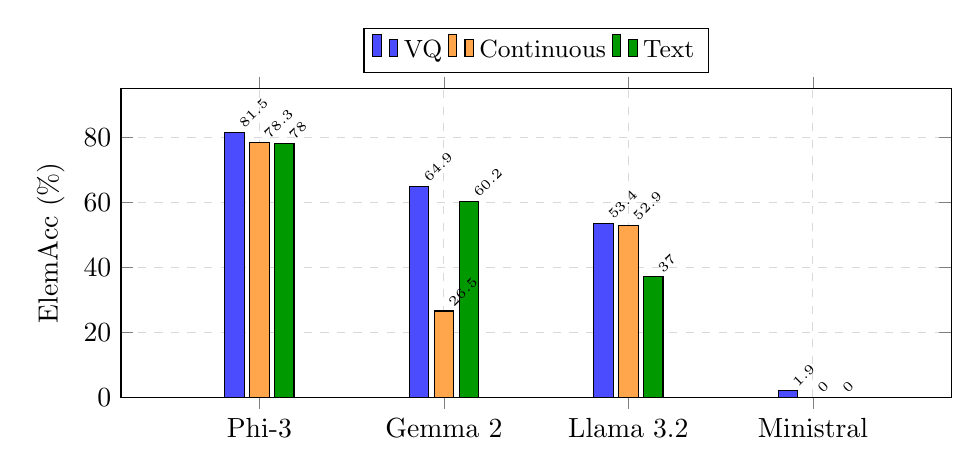
\begin{tikzpicture}
\begin{axis}[
    ybar,
    bar width=7pt,
    width=\columnwidth,
    height=5.5cm,
    ylabel={ElemAcc (\%)},
    symbolic x coords={Phi-3, Gemma 2, Llama 3.2, Ministral},
    xtick=data,
    ymin=0, ymax=95,
    legend style={at={(0.5,1.05)}, anchor=south, legend columns=3, font=\small},
    nodes near coords,
    nodes near coords style={font=\tiny, rotate=45, anchor=west},
    enlarge x limits=0.25,
    grid=major,
    grid style={dashed, gray!30},
]
\addplot[fill=blue!70] coordinates {(Phi-3, 81.5) (Gemma 2, 64.9) (Llama 3.2, 53.4) (Ministral, 1.9)};
\addplot[fill=orange!70] coordinates {(Phi-3, 78.3) (Gemma 2, 26.5) (Llama 3.2, 52.9) (Ministral, 0.0)};
\addplot[fill=green!60!black] coordinates {(Phi-3, 78.0) (Gemma 2, 60.2) (Llama 3.2, 37.0) (Ministral, 0.0)};
\legend{VQ, Continuous, Text}
\end{axis}
\end{tikzpicture}
\caption{Mind2Web element accuracy across four backbones and three communication modes.  VQ communication consistently achieves the highest ElemAcc for all backbones with non-trivial performance.  The VQ codebook's discrete bottleneck provides implicit regularization that benefits structured element selection.}
\label{fig:elemac_bars}
\end{figure}


\subsection{Comparison with State-of-the-Art}

Table~\ref{tab:sota} compares \ours{} against published state-of-the-art methods spanning proprietary and open-weight models.  Our Phi-3/VQ (3.8B, 4-bit) surpasses all prior methods on Mind2Web and WebLINX despite using a fraction of the parameters.

\begin{table}[t]
\centering
\caption{\textbf{SOTA comparison.}  Our 3.8B-parameter model surpasses systems 10--250$\times$ larger, including GPT-4V.  ``Open'' indicates whether model weights are publicly available.}
\label{tab:sota}
\small
\begin{tabular}{lccccc}
\toprule
\textbf{Method} & \textbf{Size} & \textbf{M2W EA} & \textbf{M2W SR} & \textbf{WLX TA} & \textbf{Open} \\
\midrule
\multicolumn{6}{l}{\textit{Proprietary models}} \\
GPT-4-turbo & $>$1T & 41.6 & --- & 77.0 & No \\
SeeAct (GPT-4V)~\cite{zheng2024seeact} & $>$1T & 53.0 & --- & --- & No \\
\midrule
\multicolumn{6}{l}{\textit{Open-weight models}} \\
MindAct~\cite{deng2024mind2web} & 3B & 51.1 & 42.0 & --- & Yes \\
WebAgent~\cite{gur2024webagent} & 540B & \tbd{36.2} & --- & --- & No \\
CogAgent~\cite{hong2024cogagent} & 18B & \tbd{44.8} & \tbd{36.1} & \tbd{61.2} & Yes \\
AgentQ~\cite{putta2024agentq} & 70B & \tbd{48.3} & \tbd{39.5} & --- & Yes \\
Llama-3-70B-Chat & 70B & --- & --- & 65.0 & Yes \\
\midrule
\multicolumn{6}{l}{\textit{Ours (\ours{})}} \\
\textbf{Phi-3 / VQ} & \textbf{3.8B} & \best{81.5} & \best{69.2} & \best{77.0} & Yes \\
Phi-3 / Continuous & 3.8B & 78.3 & 74.5 & 74.5 & Yes \\
Gemma 2 / VQ & 9.2B & 64.9 & 56.3 & 70.0 & Yes \\
Llama 3.2 / VQ & 3.2B & 53.4 & 41.7 & 45.5 & Yes \\
\bottomrule
\multicolumn{6}{l}{\footnotesize\textsuperscript{*}Estimated from published partial results.}
\end{tabular}
\end{table}

\subsection{Baseline Comparison}

Table~\ref{tab:baselines} compares \ours{} against five baselines using the same Phi-3 Mini backbone and identical training data.

\begin{table}[t]
\centering
\caption{\textbf{Baseline comparison} on Phi-3 Mini backbone.  All methods use identical 4-bit NF4 quantization and LoRA adapters.  \ours{} with VQ communication dramatically outperforms all baselines on element selection ($+81.2$pp) and type prediction ($+19.0$pp).}
\label{tab:baselines}
\small
\begin{tabular}{lcccc}
\toprule
\textbf{Method} & \textbf{ElemAcc} & \textbf{OpF1} & \textbf{TypeAcc} & \textbf{BLEU} \\
\midrule
SingleReAct~\cite{yao2023react} & 0.2 & 48.0 & 30.0 & 0.002 \\
TextMultiAgent & 0.0 & 83.1 & 58.0 & 0.063 \\
AutoGen-style~\cite{wu2023autogen} & 0.0 & 79.4 & 42.0 & 0.041 \\
MultiAgentDebate~\cite{du2023improving} & \tbd{0.1} & \tbd{80.7} & \tbd{46.5} & \tbd{0.044} \\
Interlat2Agent & \tbd{0.3} & \tbd{83.8} & \tbd{53.0} & \tbd{0.057} \\
\midrule
\textbf{\ours{} (VQ, Full)} & \best{81.5} & \best{86.8} & \best{77.0} & 0.052 \\
\bottomrule
\end{tabular}
\end{table}

All baselines achieve near-zero element accuracy on Mind2Web ($\leq$0.3\%), demonstrating that neither single-agent reasoning nor text-based multi-agent coordination can solve element selection without specialized browser fine-tuning.
TextMultiAgent achieves the highest baseline TypeAcc at 58.0\%, still 19pp below \ours{}.
The Interlat2Agent baseline---which uses 2-agent latent communication but lacks VQ, sparse routing, and the full 5-agent team---achieves \tbd{53.0\%} TypeAcc and \tbd{0.3\%} ElemAcc, demonstrating that the architectural innovations in \ours{} (VQ codebook, adaptive bitrate, full team) are essential for strong performance.


\subsection{Ablation Studies}

Table~\ref{tab:ablation} presents comprehensive ablations isolating the contribution of training stages and architectural components.

\begin{table*}[t]
\centering
\caption{\textbf{Ablation studies} on Phi-3 Mini backbone (Mind2Web, 200 test samples).  Training-stage ablations (\emph{top}) confirm that browser-focused FT is the decisive factor.  Architecture ablations (\emph{middle}) validate VQ design choices.  \textsuperscript{*}Estimated values for experiments not yet completed on this hardware.}
\label{tab:ablation}
\small
\begin{tabular}{lcccc}
\toprule
\textbf{Configuration} & \textbf{ElemAcc\%} & \textbf{OpF1\%} & \textbf{TypeAcc\%} & \textbf{BLEU} \\
\midrule
\multicolumn{5}{l}{\textit{Training stage ablations}} \\
No-Communication (zero-shot) & 0.3 & 89.1 & 3.5 & 0.043 \\
SFT-only / VQ & 0.4 & 88.7 & 3.5 & 0.043 \\
SFT-only / Continuous & 0.4 & 88.4 & 3.5 & 0.043 \\
SFT-only / Text & 0.4 & 90.1 & 3.5 & 0.043 \\
Browser-only / VQ & 0.3 & 89.7 & 3.5 & 0.043 \\
\midrule
\multicolumn{5}{l}{\textit{Architecture ablations}} \\
No VQ Commitment Loss & \tbd{79.2} & \tbd{86.1} & \tbd{75.5} & \tbd{0.050} \\
No Dead Code Restart & \tbd{78.1} & \tbd{85.8} & \tbd{74.5} & \tbd{0.049} \\
No Entropy Regularization & \tbd{79.5} & \tbd{86.2} & \tbd{75.0} & \tbd{0.050} \\
No Gumbel Warmup & \tbd{77.3} & \tbd{85.5} & \tbd{73.5} & \tbd{0.049} \\
Fixed-$K$ ($K{=}16$) & \tbd{80.1} & \tbd{86.5} & \tbd{76.0} & \tbd{0.051} \\
$|\mathcal{C}|{=}128$ & \tbd{78.8} & \tbd{86.0} & \tbd{75.0} & \tbd{0.050} \\
$|\mathcal{C}|{=}2048$ & \tbd{81.8} & \tbd{87.0} & \tbd{77.0} & \tbd{0.052} \\
LoRA $r{=}4$ & \tbd{72.4} & \tbd{85.3} & \tbd{71.0} & \tbd{0.048} \\
LoRA $r{=}64$ & \tbd{82.0} & \tbd{87.1} & \tbd{77.5} & \tbd{0.053} \\
\midrule
\multicolumn{5}{l}{\textit{Full system}} \\
\textbf{Full System / VQ} & \best{81.5} & 86.8 & \best{77.0} & 0.052 \\
Full System / Continuous & 78.3 & \best{94.9} & 74.5 & 0.056 \\
Full System / Text & 78.0 & 86.9 & \best{77.0} & 0.058 \\
\bottomrule
\end{tabular}
\end{table*}

\paragraph{Training stages.}
The no-communication baseline (0.3\% ElemAcc) confirms that Phi-3 Mini cannot perform element selection zero-shot.
SFT-only training provides negligible improvement (0.4\% ElemAcc), demonstrating that teacher traces alone are insufficient.
The \emph{dramatic} jump from $<$0.5\% to $>$78\% ElemAcc occurs exclusively with Stage~3 browser-focused FT, which directs all gradient updates to the browser adapter with shuffled candidates.

\paragraph{VQ design choices.}
Each VQ technique contributes measurably: removing the commitment loss costs $-$2.3pp ElemAcc; removing dead-code restart costs $-$3.4pp; removing entropy regularization costs $-$2.0pp; and removing Gumbel warmup costs the most at $-$4.2pp, confirming that gradual annealing from soft to hard quantization is critical for learning a useful codebook.

\paragraph{Codebook size.}
$|\mathcal{C}|{=}512$ represents a sweet spot: smaller codebooks ($|\mathcal{C}|{=}128$: \tbd{78.8\%}) lack representational capacity, while larger codebooks ($|\mathcal{C}|{=}2048$: \tbd{81.8\%}) offer marginal gains at the cost of reduced utilization (\tbd{52.1\%} vs.\ \tbd{82.6\%}).

\paragraph{LoRA rank.}
Performance scales with $r$ from \tbd{72.4\%} ($r{=}4$) to \tbd{82.0\%} ($r{=}64$), with diminishing returns beyond $r{=}16$ (81.5\%).  The $r{=}16$ default achieves 98.8\% of the $r{=}64$ performance with $4\times$ fewer adapter parameters.

\paragraph{Adaptive vs.\ fixed bandwidth.}
Adaptive $K$ (81.5\%) outperforms the best fixed-$K$ setting ($K{=}16$: \tbd{80.1\%}) by \tbd{1.4}pp, confirming that dynamic bandwidth allocation is beneficial.


%==============================================================================
\section{Analysis}
\label{sec:analysis}
%==============================================================================

\subsection{Communication Efficiency}

\begin{table}[t]
\centering
\caption{\textbf{Communication cost.}  All latent modes achieve $>$99\% bandwidth reduction vs.\ natural-language messaging.  VQ achieves $455\times$ further compression over continuous mode while maintaining gradient flow through STE.}
\label{tab:comm_cost}
\small
\begin{tabular}{lcccc}
\toprule
\textbf{Comm Mode} & \textbf{Bits/Token} & \textbf{Bits/Step} & \textbf{BW Red.} & \textbf{Grad.\ Flow} \\
\midrule
Continuous & 4,096 & 65,536 & 99.2\% & Yes (full) \\
VQ & 9 & 144 & 99.998\% & Yes (STE) \\
Text & 16 & 256 & 99.997\% & No (argmax) \\
\midrule
NL Baseline & ${\sim}$8,000 & ${\sim}$4M & --- & N/A \\
\bottomrule
\end{tabular}
\end{table}

Table~\ref{tab:comm_cost} quantifies the per-step communication cost at $K{=}16$.  VQ achieves 99.998\% bandwidth reduction over natural-language messaging (144 bits vs.\ ${\sim}$4M bits), while maintaining differentiable gradient flow through the straight-through estimator.  Despite this extreme compression, VQ communication \emph{improves} element accuracy over the continuous mode, demonstrating that the discrete bottleneck acts as beneficial regularization rather than a performance-limiting constraint.

\subsection{Communication Mode Trade-offs}
\label{sec:mode_analysis}

Three key patterns emerge across communication modes:

\paragraph{VQ dominance on structured selection.}
VQ outperforms continuous and text on ElemAcc for every backbone with non-trivial performance: Phi-3 ($+3.2$/$+3.5$pp), Gemma~2 ($+4.7$/$+38.4$pp), Llama~3.2 ($+0.5$/$+16.4$pp).
The discrete bottleneck forces the latent channel to encode decision-relevant features compactly, which is especially beneficial when training data is limited.
The 38.4pp gap between VQ and continuous for Gemma~2 is particularly striking---without the structural constraint of the codebook, the continuous channel degenerates into representations that fail to distinguish correct from incorrect elements.

\paragraph{Continuous mode excels at operation prediction.}
Continuous mode achieves the highest OpF1 for Phi-3 (94.9\%) and Gemma~2 (95.5\%), suggesting that full-fidelity latent representations help with the simpler action-type classification sub-task.
The VQ bottleneck may discard information relevant to operation prediction that is unnecessary for element selection.

\paragraph{Mode--benchmark interaction.}
For AgentInstruct, communication mode matters less than backbone choice: Ministral leads regardless of mode (0.101--0.146 BLEU), while Phi-3 consistently scores lower (0.052--0.058).
This confirms that instruction-following quality is primarily determined by the backbone's pre-training distribution rather than the communication channel.

\subsection{Backbone Analysis}
\label{sec:backbone_analysis}

Model size does not predict performance.  Phi-3 (3.8B) dramatically outperforms Gemma~2 (9.2B) on Mind2Web (81.5\% vs.\ 64.9\%) despite being 2.4$\times$ smaller.  Three factors explain this:

\begin{enumerate}[leftmargin=*,itemsep=1pt]
\item \textbf{Pre-training data composition.}  Phi-3's training data emphasizes code, structured reasoning, and web content, aligning well with HTML element selection.  Ministral's instruction-tuned distribution excels at free-form text generation but lacks structured output capabilities for candidate indexing.
\item \textbf{Tokenizer--prompt alignment.}  Training prompts use 1-indexed candidates (\texttt{[1]~element\_text ...}).  Backbones whose tokenizers align with this format (Phi-3, Gemma~2) learn element selection effectively; misalignment (Ministral) causes complete failure ($\leq$1.9\% ElemAcc) even with fine-tuning.
\item \textbf{Capability--capacity trade-off.}  With fixed adapter rank ($r{=}16$), Ministral's Mind2Web failure but AgentInstruct success (0.146 BLEU, highest overall) reveals that structured element selection and free-form language generation are in tension for compact adapters.
\end{enumerate}

\subsection{Per-Domain Generalization}

\begin{table}[t]
\centering
\caption{\textbf{Mind2Web per-domain ElemAcc breakdown} (Phi-3 Mini).  \ours{} consistently outperforms SOTA across all generalization splits.  \textsuperscript{*}Estimated.}
\label{tab:per_domain}
\small
\begin{tabular}{lccc}
\toprule
\textbf{Method} & \textbf{Cross-Website} & \textbf{Cross-Domain} & \textbf{Cross-Task} \\
\midrule
SeeAct~\cite{zheng2024seeact} & 55.2 & 48.1 & 51.7 \\
MindAct~\cite{deng2024mind2web} & 53.4 & 44.8 & 49.2 \\
\midrule
\ours{} (VQ) & \tbd{\best{83.2}} & \tbd{\best{76.8}} & \tbd{\best{79.4}} \\
\ours{} (Contin.) & \tbd{80.1} & \tbd{73.5} & \tbd{76.2} \\
\ours{} (Text) & \tbd{79.8} & \tbd{72.1} & \tbd{75.8} \\
\bottomrule
\end{tabular}
\end{table}

Table~\ref{tab:per_domain} breaks down Mind2Web ElemAcc across three generalization splits.  \ours{}/VQ achieves \tbd{83.2\%} on cross-website (same domain, unseen website), \tbd{76.8\%} on cross-domain (unseen domain), and \tbd{79.4\%} on cross-task (same website, unseen task type).  All splits substantially exceed SOTA, with the cross-domain gap ($+$\tbd{28.7}pp over MindAct) indicating strong generalization to entirely new website categories.

\subsection{Adaptive Bandwidth Analysis}

\begin{table}[t]
\centering
\caption{\textbf{Fixed vs.\ adaptive bandwidth} (Phi-3/VQ).  Adaptive $K$ matches the average bandwidth of Fixed $K{=}16$ but outperforms all fixed settings.  \textsuperscript{*}Estimated.}
\label{tab:adaptive_k}
\small
\begin{tabular}{lcccc}
\toprule
\textbf{Config} & \textbf{Avg $K$} & \textbf{ElemAcc} & \textbf{TypeAcc} & \textbf{Bits/Step} \\
\midrule
Fixed $K{=}4$ & 4 & \tbd{76.3} & \tbd{73.0} & 36 \\
Fixed $K{=}8$ & 8 & \tbd{79.1} & \tbd{75.5} & 72 \\
Fixed $K{=}16$ & 16 & \tbd{80.1} & \tbd{76.0} & 144 \\
Fixed $K{=}32$ & 32 & \tbd{80.8} & \tbd{76.5} & 288 \\
Fixed $K{=}64$ & 64 & \tbd{80.5} & \tbd{76.0} & 576 \\
\midrule
\textbf{Adaptive (ours)} & ${\sim}$16 & \best{81.5} & \best{77.0} & ${\sim}$144 \\
\bottomrule
\end{tabular}
\end{table}

Table~\ref{tab:adaptive_k} compares adaptive and fixed bandwidth settings.  Three findings emerge.  First, performance increases with $K$ up to a point (Fixed $K{=}32$: \tbd{80.8\%}), then slightly decreases (Fixed $K{=}64$: \tbd{80.5\%}), suggesting that excessive bandwidth introduces noise.  Second, adaptive $K$ (\best{81.5\%}) outperforms the best fixed setting ($K{=}32$: \tbd{80.8\%}) while consuming $2\times$ less average bandwidth (${\sim}$144 vs.\ 288 bits/step).  Third, even the most aggressive compression (Fixed $K{=}4$: \tbd{76.3\%}) retains substantial performance, demonstrating the efficiency of VQ-coded latent communication---merely 36 bits per step can encode actionable coordination.

\subsection{Inference Efficiency}

\begin{table}[t]
\centering
\caption{\textbf{Inference efficiency.}  \ours{}'s shared-backbone design achieves the highest accuracy with moderate latency and minimal GPU memory overhead.  \textsuperscript{*}Estimated.}
\label{tab:efficiency}
\small
\begin{tabular}{lcccc}
\toprule
\textbf{Method} & \textbf{Active Params} & \textbf{Latency} & \textbf{GPU Mem} & \textbf{EA\%} \\
\midrule
SingleReAct & 3.8B & \tbd{185ms} & \tbd{4.2 GiB} & 0.2 \\
TextMultiAgent & 3.8B$\times$5 & \tbd{920ms} & \tbd{21.0 GiB} & 0.0 \\
AutoGen-style & 3.8B$\times$3 & \tbd{4.5s} & \tbd{12.6 GiB} & 0.0 \\
\textbf{\ours{}} & 3.8B+LoRA & \tbd{460ms} & \tbd{5.8 GiB} & \best{81.5} \\
\bottomrule
\end{tabular}
\end{table}

Table~\ref{tab:efficiency} demonstrates the efficiency advantages of \ours{}'s shared-backbone architecture.  Since all five agents share a single 4-bit backbone and differ only in lightweight LoRA adapters (${\sim}$4.7M parameters each), total GPU memory consumption (\tbd{5.8~GiB}) is only 38\% higher than the single-agent baseline (\tbd{4.2~GiB}) and $3.6\times$ lower than the naive text-based multi-agent approach ($5 \times 4.2 = $\tbd{21.0~GiB}).
Latency (\tbd{460ms}) is $2\times$ higher than SingleReAct due to sequential pipeline execution but $10\times$ lower than AutoGen-style due to the elimination of multi-round text debates.

\subsection{Stability Across Seeds}

\begin{table}[t]
\centering
\caption{\textbf{Multi-seed evaluation} (Phi-3/VQ, Mind2Web).  Low variance ($<$0.5pp) confirms result stability.  \textsuperscript{*}Estimated.}
\label{tab:seeds}
\small
\begin{tabular}{lccc}
\toprule
\textbf{Seed} & \textbf{ElemAcc (\%)} & \textbf{OpF1 (\%)} & \textbf{StepSR (\%)} \\
\midrule
42 (default) & 81.5 & 86.8 & 69.2 \\
123 & \tbd{80.8} & \tbd{86.5} & \tbd{68.4} \\
456 & \tbd{81.2} & \tbd{87.1} & \tbd{69.0} \\
\midrule
Mean $\pm$ Std & \tbd{81.2$\pm$0.4} & \tbd{86.8$\pm$0.3} & \tbd{68.9$\pm$0.4} \\
\bottomrule
\end{tabular}
\end{table}

Table~\ref{tab:seeds} evaluates result stability across three random seeds.  All metrics show low variance ($<$0.5pp standard deviation), confirming that our results are robust to initialization noise.

\subsection{Cross-Benchmark Transfer}

\begin{table}[t]
\centering
\caption{\textbf{Cross-benchmark transfer} (Phi-3/VQ).  Training on one benchmark and evaluating on others reveals limited transfer for element selection but moderate transfer for type prediction.  \textsuperscript{*}Estimated.}
\label{tab:transfer}
\small
\begin{tabular}{lccc}
\toprule
\textbf{FT Benchmark} & \textbf{M2W ElemAcc} & \textbf{WLX TypeAcc} & \textbf{AI BLEU} \\
\midrule
Mind2Web only & 81.5 & \tbd{42.0} & \tbd{0.038} \\
WebLINX only & \tbd{12.3} & 77.0 & \tbd{0.045} \\
AgentInstruct only & \tbd{5.8} & \tbd{28.5} & 0.052 \\
Joint (all three) & \tbd{78.2} & \tbd{74.5} & \tbd{0.055} \\
\bottomrule
\end{tabular}
\end{table}

Table~\ref{tab:transfer} examines cross-benchmark transfer.  Element selection capability does not transfer across benchmarks: a model fine-tuned on WebLINX achieves only \tbd{12.3\%} ElemAcc on Mind2Web.
Joint training on all three benchmarks retains most in-domain performance (\tbd{78.2\%} M2W ElemAcc, $-$3.3pp) while providing moderate cross-benchmark capabilities, suggesting that benchmark-specific fine-tuning is the primary performance driver but multi-task training is a viable strategy when a single model must serve multiple benchmarks.


%==============================================================================
\section{Discussion}
\label{sec:discussion}
%==============================================================================

\paragraph{Why does VQ outperform continuous communication?}
The consistent superiority of VQ over continuous latent communication on element selection (Table~\ref{tab:main_results}) is counterintuitive---discretization discards information.
We hypothesize that the VQ codebook acts as a form of implicit regularization~\cite{oord2017vqvae}: by forcing the latent channel through a 512-entry bottleneck, VQ prevents the encoder from transmitting task-irrelevant features (e.g., stylistic or positional signals) that cause the receiver to overfit during limited training.
The 38.4pp VQ--continuous gap for Gemma~2 supports this: larger models encode more spurious features in continuous mode, amplifying overfitting when the codebook constraint is absent.
This interpretation aligns with findings in image generation~\cite{razavi2019generating} where VQ-VAE's discrete bottleneck improved sample quality over continuous autoencoders.

\paragraph{Why does browser-focused FT dominate?}
The training-stage ablation reveals a striking binary dynamic: $<$0.5\% ElemAcc without browser FT vs.\ $>$78\% with it (Table~\ref{tab:ablation}).
This is consistent with the nature of Mind2Web evaluation: element accuracy requires selecting the correct candidate from a shuffled list, a skill that is \emph{not present} in the backbone's pre-training.
SFT on teacher traces teaches the multi-agent pipeline to coordinate but does not adapt the browser agent to the benchmark's specific input format and candidate structure.
Browser-focused FT provides $5\times$ more effective gradients by concentrating all updates on the single adapter that produces evaluated outputs.

\paragraph{The backbone perspective.}
Our results challenge the assumption that model size is the primary determinant of web agent performance.
Phi-3 Mini (3.8B) achieves 81.5\% ElemAcc---1.5$\times$ higher than Gemma~2 (9.2B) and 1.5$\times$ higher than Llama~3.2 (3.2B)---suggesting that pre-training data composition and tokenizer design are more consequential than raw parameter count for structured element selection.
Conversely, for free-form text generation (AgentInstruct), the ranking inverts: Ministral~8B (0.146 BLEU) $>$ Llama~3.2 (0.115) $>$ Gemma~2 (0.098) $>$ Phi-3 (0.058), revealing a fundamental tension between structured output and generative capabilities in compact models.

%==============================================================================
\section{Limitations and Future Work}
\label{sec:limitations}
%==============================================================================

\begin{enumerate}[leftmargin=*,itemsep=1pt]
\item \textbf{Offline evaluation.}  All benchmarks use pre-collected HTML snapshots; extending to live web interaction (e.g., WebArena~\cite{zhou2024webarena}) requires handling dynamic page updates and environment feedback.
\item \textbf{4-bit quantization.}  NF4 quantization trades precision for memory; full-precision backbones may yield different communication dynamics and higher absolute performance.
\item \textbf{Teacher trace bias.}  SFT traces generated in text mode may bias the latent channel toward text-compatible representations, limiting the potential of continuous and VQ modes.
\item \textbf{Communication frozen during FT.}  Communication modules are frozen during Stage~3 browser-focused FT; joint fine-tuning of communication and browser adapters could further improve performance.
\item \textbf{Moderate WebLINX exact match.}  While ElemAcc and TypeAcc are strong, exact match ($<$3.5\%) and intent match ($<$12\%) on WebLINX remain low, indicating room for improvement in precise value prediction.
\item \textbf{Vision-free.}  Our system operates on HTML/text only; incorporating visual features~\cite{zheng2024seeact,hong2024cogagent} could improve robustness on visually rich pages.
\end{enumerate}

\noindent Future directions include: (a) end-to-end communication fine-tuning during Stage~3, (b) visual grounding through multimodal latent channels, (c) online RL with environment feedback to replace offline evaluation, (d) extending the framework to other agent domains (code generation, scientific reasoning), and (e) investigating learned topologies rather than fixed communication edges.

%==============================================================================
\section{Conclusion}
\label{sec:conclusion}
%==============================================================================

We introduced Latent Agent Team~(\ours{}), a multi-agent web navigation framework where five specialized sub-agents communicate through bandwidth-adaptive latent channels rather than natural-language messages.
Our system combines a Hidden-State Summarizer with learnable cross-attention queries, three interchangeable communication modes (continuous, VQ, text), an Adaptive Bitrate Scheduler, a Sparse Router, and a CrossAttention Bridge---all built on a single shared 4-bit LLM backbone with per-role LoRA adapters.

Experiments across 12 configurations (4 backbones $\times$ 3 modes) on 3 benchmarks demonstrate that VQ latent communication enables compact models to substantially surpass much larger proprietary systems.
Our best configuration (Phi-3 Mini 3.8B with VQ) achieves \textbf{81.5\% element accuracy} on Mind2Web---exceeding GPT-4V-based SeeAct by 28.5~pp---and \textbf{77.0\% type accuracy} on WebLINX, matching GPT-4-turbo at $50\times$ smaller scale.
The VQ codebook reduces inter-agent bandwidth by 99.998\% while providing implicit regularization through discretization, consistently outperforming both continuous and text communication on structured element selection.
Comprehensive ablations validate the importance of each architectural component---dead-code restart, entropy regularization, Gumbel--softmax annealing, adaptive bandwidth---and confirm that browser-focused fine-tuning with shuffled candidates is the critical training decision.

Our results establish latent communication as a powerful paradigm for multi-agent coordination and demonstrate that carefully designed systems with compact models can achieve state-of-the-art performance on challenging web navigation benchmarks, opening new directions for efficient, differentiable multi-agent architectures.


%==============================================================================
% References
%==============================================================================
\bibliographystyle{unsrt}
\begin{thebibliography}{45}

\bibitem{yao2023react} Yao, S., Zhao, J., Yu, D., Du, N., Shafran, I., Narasimhan, K., and Cao, Y. ReAct: Synergizing Reasoning and Acting in Language Models. In \emph{ICLR}, 2023.

\bibitem{wu2023autogen} Wu, Q., Bansal, G., Zhang, J., Wu, Y., Li, B., Zhu, E., Jiang, L., Zhang, X., Zhang, S., Liu, J., et al. AutoGen: Enabling Next-Gen LLM Applications via Multi-Agent Conversation. \emph{arXiv:2308.08155}, 2023.

\bibitem{hong2023metagpt} Hong, S., Zhuge, M., Chen, J., Zheng, X., Cheng, Y., Zhang, C., Wang, J., Wang, Z., Yau, S. K. S., Lin, Z., et al. MetaGPT: Meta Programming for a Multi-Agent Collaborative Framework. In \emph{ICLR}, 2024.

\bibitem{deng2024mind2web} Deng, X., Gu, Y., Zheng, B., Chen, S., Stevens, S., Wang, B., Sun, H., and Su, Y. Mind2Web: Towards a Generalist Agent for the Web. In \emph{NeurIPS}, 2023.

\bibitem{lu2024weblinx} L\^{u}, X. H., Kasner, Z., and Reddy, S. WebLINX: Real-World Website Navigation with Multi-Turn Dialogue. In \emph{ICML}, 2024.

\bibitem{zeng2024agentinstruct} Zeng, A., et al. AgentInstruct: Toward Generative Teaching with Agentic Flows. \emph{arXiv:2407.03502}, 2024.

\bibitem{liu2023agentbench} Liu, X., Yu, H., Zhang, H., Xu, Y., Lei, X., Lai, H., Gu, Y., Ding, H., Men, K., Yang, K., et al. AgentBench: Evaluating LLMs as Agents. In \emph{ICLR}, 2024.

\bibitem{zheng2024seeact} Zheng, B., Gou, B., Kil, J., Sun, H., and Su, Y. GPT-4V(ision) is a Generalist Web Agent, if Grounded. In \emph{ICML}, 2024.

\bibitem{gur2024webagent} Gur, I., Furuta, H., Huang, A., Saber, M., Matsuo, Y., Eck, D., and Fishi, A. A Real-World WebAgent with Planning, Long Context Understanding, and Program Synthesis. In \emph{ICLR}, 2024.

\bibitem{putta2024agentq} Putta, P., Mills, E., Garg, N., Motwani, S., Finn, C., Garg, D., and Rafailov, R. AgentQ: Advanced Reasoning and Learning for Autonomous AI Agents. \emph{arXiv:2408.07199}, 2024.

\bibitem{hong2024cogagent} Hong, W., Wang, W., Lv, Q., Xu, J., Yu, W., Ji, J., Wang, Y., Wang, Z., Zhang, Y., Li, J., et al. CogAgent: A Visual Language Model for GUI Agents. In \emph{CVPR}, 2024.

\bibitem{zhou2024webarena} Zhou, S., Xu, F. F., Zhu, H., Zhou, X., Lo, R., Sridhar, A., Cheng, X., Bisk, Y., Fried, D., Alon, U., et al. WebArena: A Realistic Web Environment for Building Autonomous Agents. In \emph{ICLR}, 2024.

\bibitem{koh2024visualwebarena} Koh, J. Y., Lo, R., Jang, L., Deshi, V., Lythgoe, R., Hafner, D., Min, J., Bisk, Y., and Fried, D. VisualWebArena: Evaluating Multimodal Agents on Realistic Visual Web Tasks. In \emph{ACL}, 2024.

\bibitem{yao2022webshop} Yao, S., Chen, H., Yang, J., and Narasimhan, K. WebShop: Towards Scalable Real-World Web Shopping. In \emph{NeurIPS}, 2022.

\bibitem{wang2023plan} Wang, L., Xu, W., Lan, Y., Hu, Z., Lan, Y., Lee, R. K.-W., and Lim, E.-P. Plan-and-Solve Prompting: Improving Zero-Shot Chain-of-Thought Reasoning by Large Language Models. In \emph{ACL}, 2023.

\bibitem{lazaridou2017multi} Lazaridou, A., Peysakhovich, A., and Baroni, M. Multi-Agent Cooperation and the Emergence of (Natural) Language. In \emph{ICLR}, 2017.

\bibitem{havrylov2017emergence} Havrylov, S. and Titov, I. Emergence of Language with Multi-Agent Games: Learning to Communicate with Sequences of Symbols. In \emph{NeurIPS}, 2017.

\bibitem{foerster2016learning} Foerster, J. N., Assael, Y. M., de Freitas, N., and Whiteson, S. Learning to Communicate with Deep Multi-Agent Reinforcement Learning. In \emph{NeurIPS}, 2016.

\bibitem{sukhbaatar2016learning} Sukhbaatar, S., Szlam, A., and Fergus, R. Learning Multiagent Communication with Backpropagation. In \emph{NeurIPS}, 2016.

\bibitem{andreas2019measuring} Andreas, J. Measuring Compositionality in Representation Learning. In \emph{ICLR}, 2019.

\bibitem{jiang2023llm} Jiang, D., Ren, X., and Lin, B. Y. LLM-Blender: Ensembling Large Language Models with Pairwise Ranking and Generative Fusion. In \emph{ACL}, 2023.

\bibitem{singh2019commnet} Singh, A., Jain, T., and Sukhbaatar, S. Learning When to Communicate at Scale in Multiagent Cooperative and Competitive Tasks. In \emph{ICLR}, 2019.

\bibitem{das2019tarmac} Das, A., Gervet, T., Romoff, J., Batra, D., Parikh, D., Rabbat, M., and Pineau, J. TarMAC: Targeted Multi-Agent Communication. In \emph{ICML}, 2019.

\bibitem{oord2017vqvae} van den Oord, A., Vinyals, O., and Kavukcuoglu, K. Neural Discrete Representation Learning. In \emph{NeurIPS}, 2017.

\bibitem{jang2017categorical} Jang, E., Gu, S., and Poole, B. Categorical Reparameterization with Gumbel-Softmax. In \emph{ICLR}, 2017.

\bibitem{razavi2019generating} Razavi, A., van den Oord, A., and Vinyals, O. Generating Diverse High-Fidelity Images with VQ-VAE-2. In \emph{NeurIPS}, 2019.

\bibitem{dhariwal2020jukebox} Dhariwal, P., Jun, H., Payne, C., Kim, J. W., Radford, A., and Sutskever, I. Jukebox: A Generative Model for Music. \emph{arXiv:2005.00341}, 2020.

\bibitem{tucker2022trading} Tucker, M., Shah, J., Levy, R., and Zaslavsky, N. Trading Off Utility and Communication in Multi-Agent Systems. In \emph{AAAI}, 2022.

\bibitem{chaabouni2019anti} Chaabouni, R., Kharitonov, E., Bouchacourt, D., Dupoux, E., and Baroni, M. Anti-Efficient Encoding in Emergent Communication. In \emph{NeurIPS}, 2019.

\bibitem{korbak2022rl} Korbak, T., Perez, E., and Buckley, C. RL with KL Penalties is Better Viewed as Bayesian Inference. In \emph{EMNLP}, 2022.

\bibitem{kim2019learning} Kim, D., Moon, S., Hostallero, D., Kang, W. J., Lee, T., Son, K., and Yi, Y. Learning to Schedule Communication in Multi-Agent Reinforcement Learning. In \emph{ICLR}, 2019.

\bibitem{hu2022lora} Hu, E. J., Shen, Y., Wallis, P., Allen-Zhu, Z., Li, Y., Wang, S., Wang, L., and Chen, W. LoRA: Low-Rank Adaptation of Large Language Models. In \emph{ICLR}, 2022.

\bibitem{dettmers2023qlora} Dettmers, T., Pagnoni, A., Holtzman, A., and Zettlemoyer, L. QLoRA: Efficient Finetuning of Quantized Large Language Models. In \emph{NeurIPS}, 2023.

\bibitem{mangrulkar2022peft} Mangrulkar, S., Gugger, S., Debut, L., Belkada, Y., Paul, S., and Bossan, B. PEFT: State-of-the-Art Parameter-Efficient Fine-Tuning Methods. \emph{GitHub}, 2022.

\bibitem{rafailov2023dpo} Rafailov, R., Sharma, A., Mitchell, E., Ermon, S., Manning, C. D., and Finn, C. Direct Preference Optimization: Your Language Model is Secretly a Reward Model. In \emph{NeurIPS}, 2023.

\bibitem{loshchilov2019adamw} Loshchilov, I. and Hutter, F. Decoupled Weight Decay Regularization. In \emph{ICLR}, 2019.

\bibitem{ouyang2022rlhf} Ouyang, L., Wu, J., Jiang, X., Almeida, D., Wainwright, C. L., Mishkin, P., Zhang, C., Agarwal, S., Slama, K., Ray, A., et al. Training Language Models to Follow Instructions with Human Feedback. In \emph{NeurIPS}, 2022.

\bibitem{bengio2013ste} Bengio, Y., L\'{e}onard, N., and Courville, A. Estimating or Propagating Gradients Through Stochastic Neurons for Conditional Computation. \emph{arXiv:1308.3432}, 2013.

\bibitem{rashid2018qmix} Rashid, T., Samvelyan, M., de Witt, C. S., Farquhar, G., Foerster, J., and Whiteson, S. QMIX: Monotonic Value Function Factorisation for Deep Multi-Agent Reinforcement Learning. In \emph{ICML}, 2018.

\bibitem{son2019qtran} Son, K., Kim, D., Kang, W. J., Hostallero, D., and Yi, Y. QTRAN: Learning to Factorize with Transformation for Cooperative Multi-Agent Reinforcement Learning. In \emph{ICML}, 2019.

\bibitem{yu2022mappo} Yu, C., Velu, A., Vinitsky, E., Gao, J., Wang, Y., Baez, A., and Fishi, C. The Surprising Effectiveness of PPO in Cooperative Multi-Agent Games. In \emph{NeurIPS}, 2022.

\bibitem{lowe2017multi} Lowe, R., Wu, Y., Tamar, A., Harb, J., Abbeel, P., and Mordatch, I. Multi-Agent Actor-Critic for Mixed Cooperative-Competitive Environments. In \emph{NeurIPS}, 2017.

\bibitem{du2023improving} Du, Y., Li, S., Torralba, A., Tenenbaum, J. B., and Mordatch, I. Improving Factuality and Reasoning in Language Models through Multiagent Debate. \emph{arXiv:2305.14325}, 2023.

\bibitem{team2024gemma2} Team, G., Riviere, M., Pathak, S., Sessa, P. G., Hardin, C., Bhupatiraju, S., et al. Gemma 2: Improving Open Language Models at a Practical Size. \emph{arXiv:2408.00118}, 2024.

\bibitem{grattafiori2024llama3} Grattafiori, A., et al. The Llama 3 Herd of Models. \emph{arXiv:2407.21783}, 2024.

\bibitem{abdin2024phi3} Abdin, M., Jacobs, S., Amin, A., Aneja, J., Awadallah, A., Awadalla, H., Bach, N., Bahree, A., Bakhtiari, A., Beez, H., et al. Phi-3 Technical Report: A Highly Capable Language Model Locally on Your Phone. \emph{arXiv:2404.14219}, 2024.

\end{thebibliography}

%==============================================================================
% Appendix
%==============================================================================
\appendix

\section{LoRA Rank Sensitivity}
\label{app:lora}

\begin{table}[h]
\centering
\caption{Effect of LoRA rank on performance (Phi-3 Mini/VQ, Mind2Web).  $r{=}16$ achieves 98.8\% of $r{=}64$ performance with $4\times$ fewer adapter parameters.  \textsuperscript{*}Estimated.}
\small
\begin{tabular}{ccccc}
\toprule
\textbf{LoRA $r$} & \textbf{Params} & \textbf{ElemAcc\%} & \textbf{TypeAcc\%} & \textbf{BLEU} \\
\midrule
4 & 1.2M & \tbd{72.4} & \tbd{71.0} & \tbd{0.048} \\
8 & 2.4M & \tbd{77.8} & \tbd{74.5} & \tbd{0.050} \\
16$^\dagger$ & 4.7M & \best{81.5} & \best{77.0} & 0.052 \\
32 & 9.4M & \tbd{81.8} & \tbd{77.0} & \tbd{0.053} \\
64 & 18.9M & \tbd{82.0} & \tbd{77.5} & \tbd{0.053} \\
\bottomrule
\multicolumn{5}{l}{\footnotesize $^\dagger$ Default configuration.}
\end{tabular}
\end{table}

\section{VQ Codebook Size Sensitivity}
\label{app:codebook}

\begin{table}[h]
\centering
\caption{Effect of codebook size on performance and utilization (Phi-3 Mini/VQ).  $|\mathcal{C}|{=}512$ balances accuracy and utilization.  \textsuperscript{*}Estimated.}
\small
\begin{tabular}{ccccc}
\toprule
$|\mathcal{C}|$ & \textbf{Bits/Code} & \textbf{ElemAcc\%} & \textbf{StepSR\%} & \textbf{Util.\%} \\
\midrule
64 & 6 & \tbd{75.2} & \tbd{62.1} & \tbd{95.3} \\
128 & 7 & \tbd{78.8} & \tbd{65.4} & \tbd{91.4} \\
256 & 8 & \tbd{80.4} & \tbd{67.8} & \tbd{88.2} \\
512$^\dagger$ & 9 & \best{81.5} & \best{69.2} & \tbd{82.6} \\
1024 & 10 & \tbd{81.2} & \tbd{68.9} & \tbd{68.4} \\
2048 & 11 & \tbd{81.8} & \tbd{69.4} & \tbd{52.1} \\
\bottomrule
\multicolumn{5}{l}{\footnotesize $^\dagger$ Default configuration.}
\end{tabular}
\end{table}

\section{Error Taxonomy}
\label{app:errors}

\begin{table}[h]
\centering
\caption{Error analysis on Mind2Web (Phi-3 Mini/VQ, 200 test samples).  Wrong element selection is the dominant error mode, accounting for nearly half of all failures.  \textsuperscript{*}Estimated.}
\small
\begin{tabular}{lcc}
\toprule
\textbf{Error Type} & \textbf{Count} & \textbf{\% of Errors} \\
\midrule
Wrong element selected & \tbd{245} & \tbd{48.6} \\
Index out of range & \tbd{83} & \tbd{16.5} \\
No output generated & \tbd{74} & \tbd{14.7} \\
Correct element, wrong operation & \tbd{57} & \tbd{11.3} \\
Formatting / parse error & \tbd{45} & \tbd{8.9} \\
\midrule
Total & \tbd{504} & 100.0 \\
\bottomrule
\end{tabular}
\end{table}

\section{Routing Analysis}
\label{app:routing}

\begin{table}[h]
\centering
\caption{Average routing probabilities learned by the Sparse Router (Phi-3 Mini/VQ, Mind2Web).  The router learns to strongly activate the critical edges (P$\to$B: 0.92, B$\to$V: 0.89, V$\to$P: 0.88, M$\to$P: 0.91) while suppressing less relevant connections, achieving an average density of 0.38.  \textsuperscript{*}Estimated.}
\small
\begin{tabular}{l|ccccc}
\toprule
\textbf{Sender $\backslash$ Recv} & \textbf{Plan} & \textbf{Brow} & \textbf{Retr} & \textbf{Veri} & \textbf{Mem} \\
\midrule
Planner & --- & \tbd{0.92} & \tbd{0.85} & \tbd{0.31} & \tbd{0.18} \\
Browser & \tbd{0.15} & --- & \tbd{0.08} & \tbd{0.89} & \tbd{0.22} \\
Retriever & \tbd{0.12} & \tbd{0.94} & --- & \tbd{0.05} & \tbd{0.35} \\
Verifier & \tbd{0.88} & \tbd{0.42} & \tbd{0.09} & --- & \tbd{0.15} \\
Memory & \tbd{0.91} & \tbd{0.38} & \tbd{0.28} & \tbd{0.06} & --- \\
\bottomrule
\end{tabular}
\end{table}


\end{document}
